\begin{frame}{Introducción}
\justifying
Comenzamos el capítulo con una discusión sobre el objeto de la ventana, que permite al programador recuperar información sobre la ventana del navegador: la URL de la página web actualmente activa, el tipo de navegador, etc. Luego pasamos a los cuadros de diálogo, que proporcionan un medio crudo, pero efectivo, para obligar al usuario a responder una pregunta. Introducimos la declaración if para hacer cosas diferentes, dependiendo de la respuesta del usuario a una pregunta. Luego hablamos de cadenas y números. Para obligar a los usuarios a proporcionar información que tenga sentido, describimos técnicas de validación de restricción de entrada. Finalmente, hablamos de varios operadores que pueden usarse con la declaración if para distinguir entre diferentes situaciones.


{\tiny Web Programming with html5, css, and javascript de John Dean (2019)}
\end{frame}

\begin{frame}{Objeto Ventana 01/02}
\justifying
\begin{figure}[H]
\centering
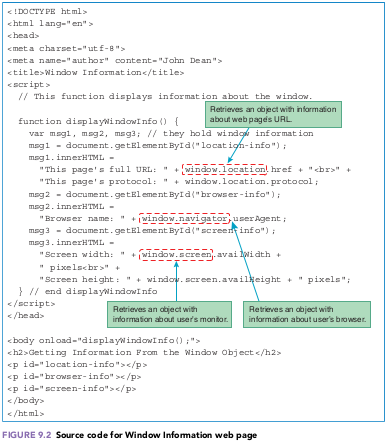
\includegraphics[scale=0.4]{Section_Files/images/Sec02/01.png}
\caption{Código fuente de una ventana.}
\end{figure}


{\tiny Web Programming with html5, css, and javascript de John Dean (2019)}
\end{frame}

\begin{frame}{Objeto Ventana 02/02}
\justifying
\begin{figure}[H]
\centering
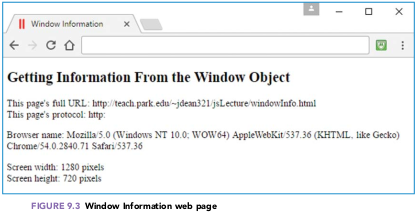
\includegraphics[scale=0.5]{Section_Files/images/Sec02/02.png}
\caption{Información de una ventana.}
\end{figure}


{\tiny Web Programming with html5, css, and javascript de John Dean (2019)}
\end{frame}